%% 電子情報通信学会 論文誌D 原著論文
%% 状態（2026-09-08）: v9．レビュー指摘への最小限の修正: (1) 推定モデルが正しい場合に提案手法の学習対象がMEPVの計算値と一致するという記述を撤回し（E[1/V] と E[V] の最適化は異なり，γ>0 では多段），5.2・5.4・6.9 を「本実験では同程度」という実証結果として記述．(2)「数値積分なし」を撤回し，学習したQ関数が置き換えるのは候補項目ごとの期待値計算であって状態の事後分散の格子計算は残ることを 5.2 に明記（あらまし・6.2・むすびの表現も修正）．v8．表2〜6の太字は表示桁（小数3桁）で列の最小値と等しい値すべて（make_tables.py の規則．2026-09-08 にコード整理と同時に統一．数値は不変）．参照報酬（参照能力値における情報量）を提案の変種・比較条件から削除（表3の感度分析にのみ残す），付録1から参照報酬関連を削除．v7．参照報酬を提案手法の変種として5.2節に移動，「較正」の語を廃止，5.5節（計算量）を削除，解釈境界を6.9節「考察」に再構成，表6に提案（参照報酬）を追加．v6．MEPG（本研究で定義した最大期待精度増分法）を全体から削除し，比較対象を MEPV に置き換え（ユーザー指示）．v5．ユーザーの1章の改訂と指示（実験固有の記述を6章へ移動，項目選択規則・推定モデル／データ生成モデルの用語統一，
%%   真の能力に関する言及と「実装可能」「信念状態」の廃止，6.7節の対照条件の削除）を反映して推敲．v4（2026-09-07）: ユーザー指示による簡素化: 再較正規則・参照オラクル・バイアス/MAE・較正誤差の掃引を削除し，
%%   不整合実験は「データ生成モデルが推測を含む3PL，項目選択規則は真の a,b の2PLM」の1ケースに限定．第2段階（HistoryDQN）と第3段階（MIRTDQN）の
%%   検討は付録に要約（転記元は appendix_sources/ に保存した集計ファイル）．v3 以前の原稿と archive は 2026-09-07 のフォルダ再編で削除済み．
%% 仮題である．
%% 転記元: ../Experiments/results/{main,sensitivity,state,ablation}（make_tables.py），
%%   ../Experiments/results/guess（make_tables.py guess），results/selection（analyze_selection.py），results/cost（benchmark_cost.py）
%% 実行コマンド: ../Experiments/README.md の「実行」を参照
%% 投稿版には含めない作業メモ: v1（2026-09-04 19:52）への外部レビュー（Codex）で指摘された
%%   報酬定義の不一致，下限の過剰主張，状態の非マルコフ性，Huber損失，指標の取り違え，乱数の重複を
%%   本版で修正した（v1・v2 の資料は 2026-09-07 に削除）．
\documentclass[paper]{ieicej}
\usepackage[dvipdfmx]{graphicx,xcolor}
\usepackage{otf}% 編集環境が非JIS文字（−，\UTF{2264}，\UTF{00B5} など）を \UTF{xxxx} に変換して保存しても組版できるようにする
\usepackage[fleqn]{amsmath}
\usepackage{newtxtext}% 英数字フォントの設定を変更しないでください
\usepackage[varg]{newtxmath}% 英数字フォントの設定を変更しないでください
\usepackage{bm}
\usepackage{color}

\setcounter{page}{1}

\field{D}
\jtitle{推定値の不確実性を考慮した状態と報酬に基づく深層強化学習型コンピュータ適応型テストの項目選択}
\etitle{Deep Reinforcement Learning Item Selection for Computerized Adaptive Testing Based on a State and a Reward Reflecting the Uncertainty of the Ability Estimate}
\authorlist{%
 \authorentry[uto@ai.lab.uec.ac.jp]{宇都 雅輝}{Masaki Uto}{UECdaigakuin}\MembershipNumber{1202618}
}
\affiliate[UECdaigakuin]{電気通信大学大学院情報理工学研究科，調布市}{The University of Electro-Communications, Chofu-shi, 182-8585, Japan}
\jalcdoi{???????????}

\begin{document}
\begin{abstract}
%% あらまし: v5（2026-09-08 推敲）．
コンピュータ適応型テストでは，受験者の能力推定値に応じて次に出題する項目を逐次的に選択する．近年，項目選択を逐次決定問題として定式化し，深層Q学習により選択方策を学習する方法が提案され，最大情報量法を上回る推定精度が報告されている．しかし，この方法には，Q関数の全パラメータに課される非負制約が価値関数の形を制限すること，能力推定値だけを状態とするため状態の遷移が一意に定まらないこと，及び報酬が最大情報量法の項目選択規準と一致するため推定値の不確実性を報酬に反映できないことという問題がある．本論文では，最尤推定値，テストの進行度，事後分散からなる状態と，事後精度の増分という推定値の不確実性を考慮した報酬を用い，パラメータに制約を課さない深層Q学習型の項目選択法を提案する．2パラメータロジスティックモデルに基づくシミュレーション実験により，提案手法がテスト序盤で最大情報量法を上回り，事後分布に基づく解析的な項目選択規則と同等の精度を，候補項目ごとの期待値計算を学習したQ関数で置き換えて達成すること，既存手法の劣化の決定的な要因が非負制約と学習設定であること，及びデータ生成モデルが推測を含む場合には実際の反応から学習した提案手法が解析的な項目選択規則を小さいながら一貫して上回ることを示す．
\end{abstract}
\begin{keyword}
コンピュータ適応型テスト，項目反応理論，項目選択，強化学習，深層Q学習
\end{keyword}
\maketitle

\section{まえがき}\label{sec:intro}

近年，受験者ごとに出題する項目を適応的に変えるコンピュータ適応型テスト（computerized adaptive testing; CAT）が，資格試験や学力調査を含む多様な場面で利用されている~\cite{Wainer2000}．CATとは，項目反応理論に基づいて受験者の能力を逐次的に推定し，その推定値に応じて次の項目を選択する方法であり，項目固定形式のテストより少ない項目数で同等の測定精度を達成できるという利点を有する~\cite{Lord1980,Wainer2000}．

CATの中核は項目選択規則である．最も広く用いられる項目選択規則は，現在の能力推定値においてフィッシャー情報量を最大にする項目を選ぶ最大情報量法（maximum Fisher information; MFI）である~\cite{Lord1980}．しかし，テスト序盤の能力推定値は真の能力から大きく離れ得るため，その推定値で情報量を最大化しても真の能力において情報量の高い項目が選ばれるとは限らないことが指摘されてきた~\cite{ChangYing1996}．この問題を解決する項目選択規則として，反応履歴の尤度で重み付けした情報量を用いる方法~\cite{VeerkampBerger1997}や，事後分布で重み付けした情報量を用いる方法~\cite{vanderLinden1998}が提案されている．

他方で，項目選択を逐次決定問題とみなし，強化学習により選択方策を獲得する方法が近年提案されている~\cite{GhoshLan2021,WangLiuXu2024}．特にWangらは，能力推定値を状態，項目を行動，選択した項目のフィッシャー情報量を報酬とするマルコフ決定過程を定義し，深層Q学習（deep Q-network; DQN）~\cite{Mnih2015}により方策を学習する方法を提案し，シミュレーション実験においてMFIを含む既存の項目選択規則を上回る推定精度を報告している~\cite{WangLiuXu2024}．しかし，この方法には次の問題がある．（1）Q関数を近似するニューラルネットワークの全パラメータに非負制約を課すため，各項目の価値が能力推定値の単調非減少な関数に制限され，困難度が推定値に近い項目ほど価値が高いという構造を表現できない．（2）状態を能力推定値だけとするため，同じ状態と行動から異なる推定値の更新が生じ，Q関数が定義する将来価値が一意に定まらない．（3）報酬設計がMFIによる項目選択規準と一致するため，MFIと同様に推定値の不確実性を報酬に反映できない．

以上の問題を解決するために，本研究では，推定値の不確実性を考慮した状態と報酬に基づく深層Q学習型の項目選択法を提案する．提案手法の利点は次のとおりである．（1）パラメータに制約を課さないため，価値関数が困難度と推定値の対応を表現できる．（2）最尤推定値，テストの進行度，事後分散からなる状態を用いるため，同じ推定値でも不確実性が異なる状態を区別できる．（3）報酬を事後精度の増分とするため，推定値の不確実性を反映した規準を学習でき，割引率を1とすると収益がテスト終了時の事後精度に一致する．%この報酬は反応履歴と推定モデルの項目パラメータだけから計算できるため，Q関数の選択を含む学習手順の全体が真の能力を要しない．

本論文では，シミュレーション実験を通して，能力推定に利用したモデルが真のデータ生成モデルと一致する場合の提案手法の精度を，事後分布に基づく解析的な項目選択規則との比較を含めて評価する．さらに，報酬，割引率，状態表現のそれぞれについて感度分析を行い，既存手法との差分についての要因分解も行うことで，精度を左右する要素を明らかにする．さらに，能力推定に利用したモデルと真のデータ生成モデルとに乖離がある場合の精度についても評価を行う．

\section{タスク設定}\label{sec:task}

\subsection{項目反応モデル}\label{sec:model}

項目バンクは$I$個の二値項目からなる．本研究では，項目$i\in\{1,\cdots,I\}$への受験者$j\in\{1,\cdots,J\}$の正答確率が，項目反応理論の一つである，2パラメータロジスティックモデル（two-parameter logistic model; 2PLM）に従うと仮定する．2PLMに基づく正答確率は次式で定義される．
\begin{equation}
 P_i(\theta_j)=\frac{1}{1+\exp\{-a_i(\theta_j-b_i)\}}
 \label{eq:2pl}
\end{equation}
ここで，$\theta_j$は受験者$j$の能力，$a_i$は項目$i$の識別力，$b_i$は項目$i$の困難度を表す．本論文では，能力推定と項目選択に利用するこの項目反応モデルを推定モデルと呼ぶ．受験者の反応を実際に生成する過程であるデータ生成モデルは推定モデルと一致するとは限らず，両者が異なる場合を\ref{sec:misspec}と\ref{sec:misspecexp}で扱う．

2PLMに従うと，項目$i$が能力$\theta$においてもつフィッシャー情報量は次式で与えられる．
\begin{equation}
 \mathcal{I}_i(\theta)=a_i^2P_i(\theta)\{1-P_i(\theta)\}
 \label{eq:info}
\end{equation}

テスト長を$L$とし，ステップ$t\in\{1,\cdots,L\}$において受験者$j$へ出題する項目を$i_{jt}$，その反応を$u_{jt}\in\{0,1\}$と書く．ステップ$t$までの反応履歴を$h_{jt}=\{(i_{js},u_{js})\}_{s=1}^{t}$，出題した項目の集合を$S_{jt}$とし，$h_{j0}=\emptyset$，$S_{j0}=\emptyset$とする．ステップ$t$で選択可能な項目の集合は$\mathcal{B}_{jt}=\{1,\cdots,I\}\setminus S_{j,t-1}$である．ステップ$t$の終了時点における能力推定値を$\hat\theta_{jt}$と書き，テスト開始前の初期値を$\hat\theta_{j0}$と書く．

\subsection{能力推定}\label{sec:est}

ステップ$t$の終了時点で，反応履歴$h_{jt}$から能力を推定する．推定法は最尤法とし，探索範囲を有界な閉区間$[\theta_{\min},\theta_{\max}]$に限定する．対数尤度は次式である．
\begin{equation}
 \begin{aligned}
 \ell_{jt}(\theta)=\sum_{s=1}^{t}\Bigl[&u_{js}\log P_{i_{js}}(\theta)\\
 &+(1-u_{js})\log\{1-P_{i_{js}}(\theta)\}\Bigr]
 \end{aligned}
 \label{eq:loglik}
\end{equation}
2PLMの対数尤度は$\theta$について凹関数であり，その導関数
\begin{equation}
 \ell'_{jt}(\theta)=\sum_{s=1}^{t}a_{i_{js}}\{u_{js}-P_{i_{js}}(\theta)\}
 \label{eq:score}
\end{equation}
は$\theta$について狭義単調減少である．したがって，区間内の最尤推定値は，区間の中点で$\ell'_{jt}$を評価し，正なら下端を，非正なら上端を中点へ更新する二分法で求められる．

全ての反応が正答または誤答である場合，最尤推定値は有限に存在しない．この場合は先行研究~\cite{WangLiuXu2024}と同じくDoddの規則~\cite{Dodd1990}に従い，前ステップの推定値からバンクの最大困難度または最小困難度へ向けて半分だけ移動させる．すなわち，$b_{\max}=\max_ib_i$，$b_{\min}=\min_ib_i$として，
\begin{equation}
 \hat\theta_{jt}=
 \begin{cases}
  \hat\theta_{j,t-1}+\dfrac{b_{\max}-\hat\theta_{j,t-1}}{2} & \text{（全問正答）}\\[2ex]
  \hat\theta_{j,t-1}-\dfrac{\hat\theta_{j,t-1}-b_{\min}}{2} & \text{（全問誤答）}\\[2ex]
  \displaystyle\mathop{\rm arg~max}_{\theta\in[\theta_{\min},\theta_{\max}]}\ell_{jt}(\theta) & \text{（それ以外）}
 \end{cases}
 \label{eq:estimator}
\end{equation}
とする．式\eqref{eq:estimator}の推定量は，本論文で比較する全ての項目選択規則で共通に用いる．したがって，項目選択規則間の差は項目の選び方だけに帰着する．また，受験者$j$の$L$個の反応全てから式\eqref{eq:estimator}で求めた推定値$\tilde\theta_j=\hat\theta_{jL}$を，以下では参照能力値と呼ぶ．参照能力値は，テスト終了後に反応記録だけから計算できる量であり，\ref{sec:sensitivity}の報酬の比較で用いる．

\subsection{事後分布}\label{sec:posterior}

後述する項目選択規則のいくつかは，反応履歴を与えたときの能力の事後分布を用いる．事前分布を標準正規分布$N(0,1)$とし，$[\theta_{\min},\theta_{\max}]$上の等間隔な$G$点の格子$\{\theta_g\}$で事後分布を近似する．格子点の事後重みは
\begin{equation}
 w_{jt}(\theta_g)=\frac{\exp\{\ell_{jt}(\theta_g)\}\,\phi(\theta_g)}{\sum_{g'}\exp\{\ell_{jt}(\theta_{g'})\}\,\phi(\theta_{g'})}
 \label{eq:post}
\end{equation}
であり，$\phi$は標準正規密度である．事後平均$\mu_{jt}=\sum_gw_{jt}(\theta_g)\theta_g$，事後分散$V_{jt}=\sum_gw_{jt}(\theta_g)(\theta_g-\mu_{jt})^2$と書く．$t=0$では$w_{j0}$は事前分布の格子近似であり，$V_{j0}$は1に近い値をとる．また，事前分布を用いない尤度の正規化重みを$\tilde w_{jt}(\theta_g)=\exp\{\ell_{jt}(\theta_g)\}/\sum_{g'}\exp\{\ell_{jt}(\theta_{g'})\}$と書く．

\section{情報量に基づく項目選択}\label{sec:info}

MFIは，ステップ$t$において，前ステップの能力推定値における情報量が最大の未出題項目を選ぶ項目選択規則である~\cite{Lord1980}．
\begin{equation}
 i_{jt}=\mathop{\rm arg~max}_{i\in\mathcal{B}_{jt}}\mathcal{I}_i(\hat\theta_{j,t-1})
 \label{eq:mfi}
\end{equation}
MFIは1ステップ先の情報量だけを最大化する局所的な項目選択規則であり，$\hat\theta_{j,t-1}$が真の能力から離れているテスト序盤には，真の能力において情報量の高い項目を選ぶとは限らない．

推定値の不確実性を考慮する項目選択規則として，情報量を能力の分布で平均する項目選択規則が提案されている．尤度重み付き情報量法（Fisher information weighted by likelihood; FIWL）~\cite{VeerkampBerger1997}は，事前分布を置かず，反応履歴の尤度を重みとする．
\begin{equation}
 i_{jt}=\mathop{\rm arg~max}_{i\in\mathcal{B}_{jt}}\sum_{g}\tilde w_{j,t-1}(\theta_g)\,\mathcal{I}_i(\theta_g)
 \label{eq:fiwl}
\end{equation}
事後重み付き情報量法（maximum posterior-weighted information; MPWI）~\cite{vanderLinden1998}は，式\eqref{eq:post}の事後重みを用いる．
\begin{equation}
 i_{jt}=\mathop{\rm arg~max}_{i\in\mathcal{B}_{jt}}\sum_{g}w_{j,t-1}(\theta_g)\,\mathcal{I}_i(\theta_g)
 \label{eq:mpwi}
\end{equation}
反応がない$t=1$では，FIWLの重みは格子上で一様，MPWIの重みは事前分布である．更に，1ステップ先の事後分散の期待値を最小にする最小期待事後分散法（minimum expected posterior variance; MEPV）~\cite{Owen1975,vanderLinden1998}は，候補項目$i$への反応$u\in\{0,1\}$の予測確率$\pi_{i}(u)=\sum_gw_{j,t-1}(\theta_g)P_i(\theta_g)^u\{1-P_i(\theta_g)\}^{1-u}$と，反応$u$を得た後の事後分散$V_{jt}(i,u)$を用いて
\begin{equation}
 i_{jt}=\mathop{\rm arg~min}_{i\in\mathcal{B}_{jt}}\sum_{u\in\{0,1\}}\pi_i(u)\,V_{jt}(i,u)
 \label{eq:mepv}
\end{equation}
とする項目選択規則である．MEPVは候補項目ごとに二通りの反応に対する事後分布のモーメントを計算する必要があり，計算量が最も大きい．

\section{強化学習に基づく項目選択}\label{sec:rl}

\subsection{マルコフ決定過程としての定式化}\label{sec:mdp}

Wangら~\cite{WangLiuXu2024}は，受験者一人のテストを一つのエピソードとし，ステップ$t$の状態を前ステップの能力推定値$s_{jt}=\hat\theta_{j,t-1}$，行動を出題する項目$i_{jt}\in\mathcal{B}_{jt}$，報酬を選択した項目が選択時の推定値においてもつフィッシャー情報量
\begin{equation}
 r^{\rm (prev)}_{jt}=\mathcal{I}_{i_{jt}}(\hat\theta_{j,t-1})
 \label{eq:reward-prev}
\end{equation}
とするマルコフ決定過程を定義した．エピソードはステップ$L$の反応を得た時点で終了する．割引率を$\gamma\in[0,1]$とし，方策$\pi$の下での行動価値関数を$Q^\pi(s,i)=E_\pi[\sum_{k=0}^{L-t}\gamma^kr_{j,t+k}\mid s_{jt}=s,i_{jt}=i]$と定める．

\subsection{深層Q学習}\label{sec:dqn}

行動価値関数を，状態を入力とし各項目の価値を並べた$I$次元ベクトルを出力する全結合ニューラルネットワーク$Q(s,\cdot;\bm{w})$で近似する．ネットワークは隠れ層2層からなり，活性化関数をReLUとする．
\begin{equation}
 Q(s,\cdot;\bm{w})=W_3\,\phi\!\left(W_2\,\phi(W_1s+\bm{c}_1)+\bm{c}_2\right)+\bm{c}_3
 \label{eq:qnet}
\end{equation}
ここで，$\phi(x)=\max(x,0)$を要素ごとに適用し，$W_1\in\mathbb{R}^{H_1\times d}$，$W_2\in\mathbb{R}^{H_2\times H_1}$，$W_3\in\mathbb{R}^{I\times H_2}$，$\bm{c}_1\in\mathbb{R}^{H_1}$，$\bm{c}_2\in\mathbb{R}^{H_2}$，$\bm{c}_3\in\mathbb{R}^I$であり，$d$は状態の次元，$\bm{w}$は全パラメータをまとめたものである．

学習は経験再生と目標ネットワークを用いるDQN~\cite{Mnih2015}に従う．学習用の受験者の能力を$N(0,1)$から生成し，$\varepsilon$-貪欲方策で項目を選び，遷移$(s_{jt},i_{jt},r_{jt},s_{j,t+1},\delta_{jt},\mathcal{B}_{j,t+1})$を容量$N_D$の再生メモリへ格納する．ここで，$\delta_{jt}=\mathbb{1}[t=L]$は終端指示変数，$\mathcal{B}_{j,t+1}$は次状態で選択可能な項目集合である．メモリから$m$件を一様に抽出し，目標ネットワーク$Q(s,\cdot;\bm{w}^-)$による目標値
\begin{equation}
 y=r+\gamma(1-\delta)\max_{i'\in\mathcal{B}'}Q(s',i';\bm{w}^-)
 \label{eq:target}
\end{equation}
と$Q(s,i;\bm{w})$との二乗誤差の平均を損失とし，Adam~\cite{KingmaBa2015}で最小化する．目標ネットワークは$\tau$回の勾配更新ごとに同期する．評価時の方策は，未出題項目の中でQ値が最大の項目を選ぶ貪欲方策である．

Wangらは，Q値が累積情報量の期待値として非負であることを保証する目的で，全てのパラメータを各更新の際に$w\leftarrow\max(w,0)$により非負へ切り詰める．また，割引率は$\gamma\in\{0.1,0.3,0.6,0.9\}$から検証により選び，学習データ量や能力分布の影響も検討している．

\subsection{既存手法の問題点}\label{sec:gap}

まえがきで述べた問題を，以下に整理する．

第一に，全パラメータの非負制約は，Q関数の形を強く制限する．入力が符号付きスカラー$\hat\theta$であり全パラメータが非負のとき，式\eqref{eq:qnet}の各出力は$\hat\theta$について非負・単調非減少・凸であり，第1層の折れ点$-c_{1h}/W_{1h}$が全て非正であることから，$\hat\theta\ge0$では厳密に1次関数となる．このとき，困難度$b_i$の項目の価値が$\hat\theta\approx b_i$で最大となる山型の依存を表現できない．なお，Q値の形の制約だけから項目の順位付けが常に不適切になるとは言えないため，この制約の実際の影響は\ref{sec:ablation}で実測により確かめる．

第二に，能力推定値$\hat\theta$は決定過程の状態として不十分である．同じ$\hat\theta$と同じステップ数をもつ二つの反応履歴でも，尤度の形が異なれば，同じ項目へ同じ反応をしたときの更新後の推定値は異なる．例えば，識別力を1，困難度を$-1$と$1$とする2項目に1正答1誤答の履歴と，困難度を$-2$と$2$とする2項目に同じ反応をした履歴は，いずれも最尤推定値が0であるが，その後に困難度0の項目へ正答したときの推定値はそれぞれ約0.80と約1.11になる．したがって，$\hat\theta$とステップ数を与えても遷移は一意でなく，Q関数が近似すべき価値は履歴に依存する．出題済み項目を選択から除外するマスクはこの問題を解決しない．マスクはQ関数の入力に含まれないためである．

第三に，報酬の定義に関する問題である．式\eqref{eq:reward-prev}の報酬は，選択時の推定値における情報量であり，MFIの選択規準そのものである．したがって，$\gamma=0$のときQ関数は状態と行動の決定的な関数となり，学習は既知の規準を近似するだけになる．$\gamma>0$では後続の情報量が加わるが，推定値が真の能力から離れているときにその推定値で情報量を評価するというMFIの問題は，報酬の水準で引き継がれる．推定値の不確実性を報酬に反映するには，推定値の1点ではなく，その不確実性を含む量を報酬とする必要がある．

\section{提案手法}\label{sec:prop}

\subsection{推定値の不確実性を考慮した状態}\label{sec:belief}

提案手法では，ステップ$t$の状態を，最尤推定値，テストの進行度，事後分散の対数からなる3次元ベクトル
\begin{equation}
 s_{jt}=\left(\hat\theta_{j,t-1},\ \frac{t-1}{L},\ \log V_{j,t-1}\right)
 \label{eq:state}
\end{equation}
とする．$V_{j,t-1}$は式\eqref{eq:post}の事後分散である．最尤推定値は能力の位置を，事後分散は反応履歴が能力について与える不確実性を表す．\ref{sec:gap}の例では，二つの履歴の事後分散は異なるため，状態として区別される．なお，状態は反応履歴の全ての情報を保持するわけではなく，尤度の非対称性などは失われる．反応履歴をそのまま状態に含める定式化については付録1で検討する．

\subsection{推定値の不確実性を考慮した報酬}\label{sec:reward}

報酬を，反応によって事後精度（事後分散の逆数）がどれだけ増えたか
\begin{equation}
 r_{jt}=\frac{1}{V_{jt}}-\frac{1}{V_{j,t-1}}
 \label{eq:reward}
\end{equation}
とする．この報酬には次の性質がある．（1）反応履歴と推定モデルだけから計算できる．（2）割引率を$\gamma=1$とすると，エピソードの収益は$\sum_{t=1}^{L}r_{jt}=1/V_{jL}-1/V_{j0}$と伸縮し，テスト終了時の事後精度に一致する．したがって，$\gamma=1$の下での収益の期待値の最大化は，最終的な事後精度の期待値$E[1/V_{jL}]$の最大化である．なお，逆数の期待値と期待値の逆数は一致しないため，これは事後分散の期待値$E[V_{jL}]$の最小化とは同値でない．また，$\gamma<1$では途中のステップの精度増分にも重みが置かれ，最終ステップだけを目的とする定式化ではない．（3）報酬は推定値の有界性による移動を含まない．反応が予想外であれば事後分散は増え得るため，報酬は負にもなる．これに対し，参照能力値に対する推定誤差の減少量$(\hat\theta_{j,t-1}-\tilde\theta_j)^2-(\hat\theta_{jt}-\tilde\theta_j)^2$のような報酬は，収益が同様に伸縮する一方で，式\eqref{eq:estimator}の半分移動を含む推定値の変動を直接に反映する．（4）事後分散の対数減少量$\log V_{j,t-1}-\log V_{jt}$は，収益がテスト終了時の事後精度の対数に一致する同様の性質をもつが，その大きさは蓄積した精度に反比例してステップとともに減少する．式\eqref{eq:reward}と対数減少量の値の大きさは\ref{sec:selection}で実測して示し，これらの報酬との比較は\ref{sec:sensitivity}で行う．

$\gamma=0$のとき，Q関数は状態と行動を与えたときの式\eqref{eq:reward}の条件付き期待値，すなわち1ステップ先の期待事後精度増分を近似する．MEPVが1ステップ先の期待事後分散を推定モデルの下で候補項目ごとに数値積分で求めるのに対し，提案手法は，1ステップ先の期待事後精度増分を候補項目ごとの期待値計算の代わりに実際の反応から学習する．ただし，状態に含める事後分散の計算には\ref{sec:posterior}の格子上の事後分布を用いるため，学習したQ関数が置き換えるのは候補項目ごとの期待値計算であり，格子上の事後分布の計算ではない．$\gamma>0$では，後続の選択を含む複数ステップの精度増分を考慮する．なお，逆数の期待値と期待値の逆数は一致しないため，$\gamma=0$の場合でも提案手法の目的はMEPVの目的と同一ではなく，両者の選択は必ずしも一致しない．

\subsection{制約と学習}\label{sec:learning}

提案手法では，Q関数のパラメータに非負制約を課さない．式\eqref{eq:reward}の報酬は負にもなり得るため非負制約には根拠がなく，制約を課さなければ\ref{sec:gap}で述べた形の制限も生じない．学習は\ref{sec:dqn}の手順に従い，$M$人の受験者を並列に進行させ，$M$人分の遷移を格納するごとに1回の勾配更新を行う．勾配はノルムが10を超える場合に10へ縮小する．探索率は，累積受験者数$n$と学習受験者数$N$に対して
\begin{equation}
 \varepsilon(n)=\varepsilon_{\rm s}+\min\!\left(1,\frac{n}{\rho N}\right)(\varepsilon_{\rm e}-\varepsilon_{\rm s})
 \label{eq:epsilon}
\end{equation}
により線形に減少させる．一定の受験者数$N_{\rm int}$ごとに，固定した検証用受験者$N_{\rm val}$人に貪欲方策でテストを実施し，式\eqref{eq:reward}の収益$1/V_{jL}-1/V_{j0}$の平均を検証得点として算出し，学習終了後に検証得点が最大であった時点のパラメータを最終的なQ関数とする．検証得点は反応履歴と推定モデルだけから計算できる．

\subsection{実際の反応からの学習と推定モデルへの依存}\label{sec:misspec}

MFI，FIWL，MPWI，MEPVは，推定モデルとその項目パラメータが正しいという仮定の下で情報量や事後分布を計算する項目選択規則である．実際の運用では，項目パラメータは有限の反応データから推定した値であり，反応過程には推測や不注意など推定モデルに含まれない成分がある．このとき，これらの項目選択規則が計算する期待情報量や期待事後分散は，データ生成モデルの下での値と異なる．

提案手法のQ関数は，状態と行動を与えたときの報酬の条件付き期待値を，学習中にデータ生成モデルと相互作用して得た反応から学習する．報酬の式\eqref{eq:reward}は推定モデルで計算されるが，その期待値はデータ生成モデルに従う反応の分布の下で評価される．したがって，推定モデルがデータ生成モデルと異なる場合でも，提案手法が学習するのは「その項目を出題したときに推定モデルの下で実際に生じる事後精度の増分」の期待値であり，解析的な項目選択規則が計算する「推定モデルの下で生じるはずの増分」とは異なる．この差は，受験者の反応から学習するという強化学習の動機~\cite{WangLiuXu2024}が精度の改善へ結びつく経路であり，\ref{sec:misspecexp}でこの経路の有無を実験により確かめる．

この経路には留意点がある．推定モデルで計算した事後精度は実際の推定誤差そのものではないため，その期待値を正しく学んでも，推定モデルの誤りによる推定量の偏りは残る．提案手法が改善するのは項目の選び方であり，推定量の偏りではない．また，推定モデルがデータ生成モデルと一致する場合には，提案手法が学習する期待値は推定モデルの下で計算できる量であり，この経路による改善は生じない．ただし，\ref{sec:reward}で述べたとおり提案手法の目的はMEPVの目的と同一ではないため，この場合の両者の精度の関係は\ref{sec:expresult}の実験により確かめる．なお，本研究の学習はデータ生成モデルとの相互作用を仮定している．固定された過去の記録だけから学習する場合には，記録にない行動の価値の外挿という別の問題~\cite{Fujimoto2019}が生じるが，パラメータ推定に用いた反応データのように全項目への反応をもつ記録から学習する場合については付録1で検討する．

\section{シミュレーション実験}\label{sec:exp}

\subsection{実験設定}\label{sec:expsetting}

項目バンクは1種類とし，$I=500$項目の識別力を平均1.2，標準偏差0.25の正規分布から正の値が得られるまで再抽出して生成し，困難度を$N(0,1)$から生成した．評価用の受験者は反復ごとに$J=2000$人とし，真の能力を$N(0,1)$から生成した．テスト長は$L=40$とし，能力推定値の初期値$\hat\theta_{j0}$は一様分布$U(-0.5,0.5)$から生成した．最尤推定の探索範囲は$[\theta_{\min},\theta_{\max}]=[-4,4]$，二分法の反復回数は40回，事後分布の格子点数は$G=81$とした．シミュレーションにおける反応は，各受験者・各ステップについて一様乱数$\xi_{jt}\sim U(0,1)$をテストの開始前に生成しておき，$u_{jt}=\mathbb{1}[\xi_{jt}\le P_{i_{jt}}(\theta_j)]$として定めた．$\hat\theta_{j0}$と$\xi_{jt}$は評価用の乱数種のみで決まるため，同じ乱数種で評価した異なる項目選択規則は，同一の受験者と同一の乱数に直面する．これは共通乱数法による分散削減であり，項目選択規則間の差を選択方策の差として読むためのものである．実験は，項目バンクを固定したまま，評価用受験者，評価用の反応乱数，DQNの初期化・学習・検証に用いる乱数を反復ごとに変えて3回反復した．バンク，評価用受験者，学習用受験者，検証用受験者，反応乱数は，いずれも乱数種と用途識別子の組から独立に生成した乱数列を用い，用途間で乱数列が重ならないようにした．報酬と割引率の感度分析，状態表現の比較，及び要因分解は設計の選択を目的とする探索的な実験であり，反復1から3の乱数種で行った．主結果と推定モデルがデータ生成モデルと異なる場合の比較は，選択した設計を評価する確証的な実験であり，探索に用いなかった反復4から6の乱数種で行った．

比較する項目選択規則を表\ref{tab:methods}に示す．MFI，FIWL，MPWI，MEPVは\ref{sec:info}の項目選択規則である．このうちMEPVは，1ステップ先の期待事後分散を推定モデルの下で数値積分により最小化する規則であり，提案手法が事後分布に基づく解析的な項目選択規則にどこまで近づくかを検証する直接の比較対象である．既存手法は，\ref{sec:mdp}の定式化に基づくDQNであり，Wangらの論文本文の記述に従い，報酬に式\eqref{eq:reward-prev}，状態に$\hat\theta$のみ，全パラメータの非負制約，隠れ層の幅50と30，学習受験者1000人の逐次学習，再生メモリ容量1000，ミニバッチ128，目標ネットワークの同期間隔40，定数$\varepsilon=0.1$，検証間隔50人，検証用受験者200人を用いた．割引率は，Wangらが検証により選んだ候補のうち最小の0.1に固定した．本文の記述と異なる点は，項目反応モデルを3パラメータロジスティックモデルから2PLMへ，バンクを複数から単一へ簡略化したこと，Q関数の選択の規準を提案手法と同じ検証得点（当該条件の報酬の収益）としたこと，及び遷移ごとの終端判定と出題済み項目の除外を全ての条件で共通に用いたことである．したがって，既存手法の条件は先行研究の設定に基づく条件であり，公刊結果の再現ではない．

提案手法は，\ref{sec:prop}の定式化に基づき，状態を式\eqref{eq:state}，報酬を式\eqref{eq:reward}，制約なし，隠れ層の幅64と64，学習受験者$N=20000$人，並列数$M=32$，再生メモリ容量$N_D=50000$，ミニバッチ$m=128$，同期間隔$\tau=500$，学習率$10^{-3}$，探索率$(\varepsilon_{\rm s},\varepsilon_{\rm e},\rho)=(1,0.05,0.5)$，検証間隔$N_{\rm int}=2000$人，検証用受験者$N_{\rm val}=500$人とした．割引率は，\ref{sec:sensitivity}の感度分析に基づいて$\gamma=0.5$とした．各DQN条件の検証得点には当該条件の報酬の収益を用いた．

\begin{table}[t]
\centering
\caption{比較する項目選択規則}
\label{tab:methods}
\footnotesize
\setlength{\tabcolsep}{2pt}
\begin{tabular}{lll}
\hline
名称 & 項目選択規則 & 備考\\
\hline
MFI & 式\eqref{eq:mfi} & \\
FIWL & 式\eqref{eq:fiwl} & 尤度重み\\
MPWI & 式\eqref{eq:mpwi} & 事後重み\\
MEPV & 式\eqref{eq:mepv} & 1ステップ先の期待事後分散\\
既存 & DQN，報酬 式\eqref{eq:reward-prev} & 先行研究の本文の設定\\
提案 & DQN，式\eqref{eq:state}，式\eqref{eq:reward} & 制約なし\\
\hline
\end{tabular}
\end{table}

評価指標は，ステップ$t$の推定値$\hat\theta_{jt}$と真の能力$\theta_j$から計算するRMSEである．
\begin{equation}
 \mathrm{RMSE}_t=\sqrt{\frac{1}{J}\sum_{j=1}^{J}(\hat\theta_{jt}-\theta_j)^2}
 \label{eq:metrics}
\end{equation}
項目選択規則間の比較は，同じ反復の同じ受験者に対するRMSEの対応のある差により行い，3反復にわたる差の平均と範囲を報告する．反復数が3であるため統計的検定は行わず，差の符号が3反復で一致するかどうかを併せて示す．

更に，参考値として，受験者$j$の真の能力において情報量が大きい順に$L$項目を選んだときの総情報量$\mathcal{I}^*_j$から
\begin{equation}
 \mathrm{RMSE}^\dagger=\sqrt{\frac{1}{J}\sum_{j=1}^{J}\frac{1}{\mathcal{I}^*_j}}
 \label{eq:reference}
\end{equation}
を算出する．これは，真の能力を知る項目選択規則が$L$項目で得る情報量に対する不偏推定量の漸近分散から導いた参照値であり，有界な推定量の有限標本のRMSEに対する下限ではない．実際，個々の反復では実測のRMSEがこの値を下回ることがある．本論文では，この値を各項目選択規則の精度を位置付けるための目安として用い，改善の可能性を否定する根拠には用いない．

\subsection{主結果}\label{sec:expresult}

%% 転記元: results/main/mean.csv（make_tables.py main の出力 results/main/table_rows.txt），対応差は同出力．2026-09-05 転記済み（反復4-6）．
%% 参照値 0.215（反復ごとに 0.2150, 0.2153, 0.2150）．
%% 対応差（s5/s10/s40）: MPWI−MFI −0.017(3/3負)/−0.005(混在)/+0.002(3/3正)；MEPV−MFI −0.017 [−0.024,−0.009](3/3負)/−0.004(混在)/+0.002(混在)；MPWI−MEPV 全ステップ |平均| ≤0.001 混在
%%   FIWL−MFI s1 +0.138 s3 +0.031 s5 +0.017（3/3正），s10以降 平均|差|最大 0.007（s11）
%%   既存−MFI 全ステップ 3/3正，s40 +0.039 [+0.035,+0.043]
%%   提案−MFI s1 +0.027(3/3正) s3 +0.015(3/3正) s5 −0.017 [−0.021,−0.015](3/3負) s10 −0.008 [−0.025,+0.001] s20 +0.002 s40 +0.001 [−0.002,+0.003]
%%   提案−MEPV s5 −0.0005 s10 −0.0035 [−0.011,+0.001] s20 +0.0000 s40 −0.0002（いずれも混在，|平均| ≤0.004）
実験結果を表\ref{tab:main}に示す．表\ref{tab:main}は，各ステップにおけるRMSEの3反復にわたる平均を項目選択規則ごとに示したものであり，最右列は使用した項目数の反復平均である．表では，各ステップの最良値を太字で示している．

\begin{table}[t]
\centering
\caption{各ステップにおけるRMSE（反復4から6の平均）}
\label{tab:main}
\footnotesize
\setlength{\tabcolsep}{2pt}
\begin{tabular}{lcccccccc}
\hline
 & \multicolumn{7}{c}{ステップ} & \\
項目選択規則 & 1 & 3 & 5 & 10 & 20 & 30 & 40 & 項目数\\
\hline
MFI & \textbf{1.257} & \textbf{0.765} & 0.613 & 0.428 & \textbf{0.300} & \textbf{0.249} & \textbf{0.218} & 202\\
FIWL & 1.396 & 0.796 & 0.629 & 0.435 & 0.301 & 0.251 & 0.220 & 198\\
MPWI & 1.285 & 0.771 & \textbf{0.596} & 0.423 & 0.301 & \textbf{0.249} & 0.220 & 189\\
MEPV & 1.285 & 0.771 & \textbf{0.596} & 0.423 & 0.302 & \textbf{0.249} & 0.220 & 187\\
既存 & 1.282 & 0.857 & 0.695 & 0.472 & 0.340 & 0.286 & 0.258 & 72\\
提案 & 1.285 & 0.780 & \textbf{0.596} & \textbf{0.420} & 0.302 & 0.250 & 0.220 & 168\\
\hline
\end{tabular}
\end{table}

%% 結果段落の構成: 参照値との位置関係 → MFI/FIWL/MPWI/MEPV → 既存 → 提案
表\ref{tab:main}から，次のことがわかる．第一に，ステップ40のRMSEは，既存手法を除く全ての項目選択規則で0.218から0.220の範囲にあり，式\eqref{eq:reference}の参照値0.215に近い．すなわち，40項目の時点では項目選択規則間の差は小さく，差はテスト序盤から中盤に現れる．第二に，情報量に基づく項目選択規則の中では，事前分布を用いるMPWIとMEPVがステップ5でMFIを下回り，MFIとの対応差はいずれも$-0.017$（MEPVの範囲$-0.024$から$-0.009$）で3反復の全てで負である．ステップ10では平均$-0.005$と$-0.004$であるが反復により符号が変わり，ステップ20以降はMFIと0.002以内の差である．MPWIとMEPVの対応差は全てのステップで平均の絶対値が0.001以下であり，本設定では両者はほぼ同じ項目を選ぶ．事前分布を用いないFIWLはステップ1から5でMFIを上回り（ステップ5で$+0.017$，3反復の全てで正），ステップ10以降はMFIとの平均差が最大でも0.007である．

第三に，既存手法は全てのステップで3反復の全てでMFIより大きく，ステップ40の対応差は$+0.039$（範囲$+0.035$から$+0.043$）である．使用項目数は72とMFIの202の3分の1程度にとどまる．本研究の設定では，既存手法はMFIを上回らない．

第四に，提案手法は，ステップ5でMFIを下回り，対応差は$-0.017$（範囲$-0.021$から$-0.015$，MFIの0.613の約3\%に相当）と3反復の全てで負である．ステップ10では平均$-0.008$（範囲$-0.025$から$+0.001$）であり，ステップ20と40ではMFIと同等である（ステップ40の対応差$+0.001$，範囲$-0.002$から$+0.003$）．既存手法に対しては，ステップ40で0.038小さく，使用項目数も168と多い．一方，ステップ1と3では提案手法はMFIより大きく（対応差$+0.027$と$+0.015$，3反復の全てで正），この区間ではMPWIとMEPVも同様である．テスト開始直後の推定値は式\eqref{eq:estimator}の半分移動で決まる部分が大きく，事後分布に基づく項目選択規則の利点はステップ5以降に現れる．MEPVとの比較では，提案手法との対応差はステップ5から40のいずれでも平均の絶対値が0.004以下（ステップ10で$-0.004$，範囲$-0.011$から$+0.001$）で反復により符号が変わる．すなわち，提案手法は，1ステップ先の事後分布のモーメントを候補項目ごとに数値積分で求めるMEPVと同等の精度を，候補項目ごとの期待値計算の代わりに学習により達成している．

以上の結果から，推定モデルがデータ生成モデルと一致する場合には，提案手法がテスト序盤でMFIを上回り，事後分布に基づく解析的な項目選択規則と同等の精度を学習により達成することが確認できた．

\subsection{報酬関数と割引率の感度分析}\label{sec:sensitivity}

提案手法の状態と学習設定の下で，報酬を式\eqref{eq:reward}，事後分散の対数減少量$\log V_{j,t-1}-\log V_{jt}$，参照能力値における情報量$\mathcal{I}_{i_{jt}}(\tilde\theta_j)$，式\eqref{eq:reward-prev}，反応後の推定値における情報量$\mathcal{I}_{i_{jt}}(\hat\theta_{jt})$，参照能力値に対する推定誤差の減少量$(\hat\theta_{j,t-1}-\tilde\theta_j)^2-(\hat\theta_{jt}-\tilde\theta_j)^2$，及び参照能力値に対する負の二乗誤差$-(\hat\theta_{jt}-\tilde\theta_j)^2$の7種類，割引率を$\gamma\in\{0,0.5,0.9,1\}$の4水準とした計28条件を，反復1から3で実施した．いずれの報酬も反応記録だけから計算でき，参照能力値を用いる三つの報酬はエピソードの終了後に割り当てる．各条件の検証得点には当該条件の報酬の収益を用いた．

%% 転記元: results/sensitivity/mean.csv（make_tables.py sensitivity の出力 results/sensitivity/table_rows.txt）．2026-09-05 転記済み（反復1-3）．
%% MFI（反復1-3）: 0.623/0.429/0.301/0.220（MEPV の値は results/sensitivity/table_rows.txt）
%% 対応差（s5/s10/s20/s40）: 式(17)γ=0−MFI −0.028(3/3負)/−0.012(3/3負)/−0.001(混在)/+0.003 [+0.0002,+0.005](3/3正)
%%   式(17)γ=0.5−MFI −0.023(3/3負)/−0.010 [−0.016,+0.0004]/−0.001/+0.002 [+0.0003,+0.004](3/3正)
%%   γ=0−γ=0.5（式(17)）: −0.006 [−0.011,+0.0004]/−0.002/−0.0004/+0.001 いずれも混在
%%   式(13)γ=0−MFI −0.025(3/3負)/−0.008(3/3負)/+0.0001/+0.0005(3/3正)；式(12)γ=0−MFI +0.004(3/3正)/−0.002(3/3負)/−0.001/−0.003(3/3負)
%% SD@5 の最大: 対数分散減少 γ=1 0.434，参照誤差減少 γ=1 0.345；式(17) 0.062（γ=1），γ\UTF{2264}0.5 では 0.007 以下
実験結果を表\ref{tab:sensitivity}に示す．表\ref{tab:sensitivity}は，ステップ5，10，20，40におけるRMSEの3反復にわたる平均を報酬と割引率の組合せごとに示したものであり，最右列は使用した項目数の反復平均である．表では，各ステップの最良値を太字で示している．

\begin{table}[t]
\centering
\caption{報酬と割引率に対するRMSEの感度（反復1から3の平均）}
\label{tab:sensitivity}
\footnotesize
\setlength{\tabcolsep}{3pt}
\begin{tabular}{llccccc}
\hline
 & & \multicolumn{4}{c}{ステップ} & \\
報酬 & $\gamma$ & 5 & 10 & 20 & 40 & 項目数\\
\hline
提案手法（式\eqref{eq:reward}） & 0 & \textbf{0.594} & \textbf{0.416} & \textbf{0.300} & 0.223 & 170\\
 & 0.5 & 0.600 & 0.419 & \textbf{0.300} & 0.222 & 167\\
 & 0.9 & 0.665 & 0.451 & 0.311 & 0.223 & 158\\
 & 1 & 0.718 & 0.483 & 0.337 & 0.238 & 156\\
\hline
対数分散減少 & 0 & 0.598 & 0.418 & 0.303 & 0.231 & 159\\
 & 0.5 & 0.611 & 0.426 & 0.309 & 0.232 & 169\\
 & 0.9 & 0.692 & 0.457 & 0.324 & 0.239 & 157\\
 & 1 & 1.197 & 0.567 & 0.369 & 0.265 & 138\\
\hline
参照能力値FI & 0 & 0.598 & 0.421 & 0.301 & 0.221 & 193\\
 & 0.5 & 0.608 & 0.421 & 0.301 & 0.220 & 180\\
 & 0.9 & 0.664 & 0.449 & 0.310 & 0.222 & 166\\
 & 1 & 0.657 & 0.438 & 0.315 & 0.231 & 158\\
\hline
既存手法（式\eqref{eq:reward-prev}） & 0 & 0.626 & 0.427 & \textbf{0.300} & \textbf{0.217} & 199\\
 & 0.5 & 0.631 & 0.428 & 0.303 & 0.220 & 184\\
 & 0.9 & 0.672 & 0.452 & 0.310 & 0.222 & 175\\
 & 1 & 0.657 & 0.454 & 0.317 & 0.230 & 178\\
\hline
反応後推定値FI & 0 & 0.609 & 0.422 & \textbf{0.300} & 0.219 & 194\\
 & 0.5 & 0.618 & 0.426 & \textbf{0.300} & 0.222 & 187\\
 & 0.9 & 0.707 & 0.469 & 0.315 & 0.227 & 172\\
 & 1 & 0.663 & 0.451 & 0.317 & 0.231 & 168\\
\hline
参照誤差減少 & 0 & 0.790 & 0.591 & 0.455 & 0.334 & 73\\
 & 0.5 & 0.915 & 0.659 & 0.461 & 0.333 & 83\\
 & 0.9 & 1.277 & 0.813 & 0.514 & 0.356 & 99\\
 & 1 & 1.695 & 1.252 & 0.840 & 0.459 & 125\\
\hline
参照負二乗誤差 & 0 & 0.803 & 0.599 & 0.452 & 0.339 & 88\\
 & 0.5 & 0.783 & 0.598 & 0.451 & 0.329 & 110\\
 & 0.9 & 0.746 & 0.555 & 0.391 & 0.291 & 169\\
 & 1 & 0.640 & 0.485 & 0.374 & 0.285 & 146\\
\hline
\end{tabular}
\end{table}

%% 結果段落の構成: 提案報酬のγ依存 → 対数分散減少との対比 → 参照能力値FI → 推定値FI（MFI模倣）→ 誤差型報酬 → γの結論
表\ref{tab:sensitivity}から，次のことがわかる．第一に，提案する式\eqref{eq:reward}の報酬は，$\gamma=0$と$\gamma=0.5$においてステップ5と10でMFIを下回る．$\gamma=0$のMFIに対する対応差は，ステップ5で平均$-0.028$（範囲$-0.033$から$-0.024$），ステップ10で平均$-0.012$（範囲$-0.022$から$-0.003$）であり，いずれも3反復の全てで負である．ステップ20ではMFIと同等であり，ステップ40では平均$+0.003$（範囲$+0.0002$から$+0.005$）と3反復の全てでMFIをわずかに上回る．$\gamma=0.5$も同様であり，$\gamma=0$との差は全てのステップで平均の絶対値が0.006以下で反復により符号が変わる．一方，$\gamma=0.9$と$\gamma=1$では全てのステップで精度が低下し，ステップ5では0.665と0.718である．本研究では$\gamma=0.5$を採用したが，$\gamma=0$との差は認められず，割引率は0から0.5の範囲で同等，0.9以上で劣化する．なお，この選択は反復1から3の結果に基づくものであり，\ref{sec:expresult}の反復4から6における評価とは独立である．

第二に，事後分散の対数減少量を報酬とした場合は，ステップ5と10では式\eqref{eq:reward}と同程度であるが，ステップ40では0.231から0.239と劣り，$\gamma=1$ではステップ5の反復間の標準偏差が0.434に達する．この報酬の大きさは\ref{sec:selection}で示すようにステップとともに減少するため，終盤の学習信号が相対的に弱くなるという\ref{sec:reward}の見込みと整合する．ただし，本実験はこの機序を直接に測定したものではない．

第三に，参照能力値における情報量を報酬とした場合は，$\gamma=0$においてステップ5と10でMFIを下回り（対応差$-0.025$と$-0.008$，3反復の全てで負），ステップ40では0.221と式\eqref{eq:reward}と同程度である．この報酬はエピソードの終了後にしか割り当てられないが，その学習の結果は提案する報酬と同等である．一方，選択時の推定値における情報量を報酬とする式\eqref{eq:reward-prev}は，$\gamma=0$においてステップ5で3反復の全てでMFIをわずかに上回り（平均$+0.004$），ステップ40では3反復の全てでMFIをわずかに下回る（平均$-0.003$）ものの，使用項目数を含めてMFIとほぼ同じ挙動を示す．これは，\ref{sec:gap}で述べたとおり，この報酬の下でDQNがMFIを模倣することを実測で確認したものである．反応後の推定値における情報量を報酬とした場合も同様である．

第四に，参照能力値に対する推定誤差に基づく二つの報酬は，割引率によらず他の報酬より大きく劣り，ステップ40のRMSEは0.285から0.459とMFIより30\%から109\%大きく，使用項目数は73から169に減る．これらの報酬は式\eqref{eq:estimator}の半分移動を含む推定値の変動を直接に反映するため，同じ状態と行動に対する値の変動が情報量型や事後精度型の報酬より大きい．なお，情報量型と事後精度型の報酬では$\gamma\ge0.9$で一様に劣化したが，負の二乗誤差では$\gamma=1$が最良であり，割引率の影響は報酬に依存する．以上の結果から，反応記録から計算できる報酬の中では式\eqref{eq:reward}と参照能力値における情報量が同程度に有効であり，割引率は0から0.5の範囲で同等で0.9以上で劣化することが確認できた．

\subsection{状態表現の比較}\label{sec:stateexp}

提案手法の報酬と学習設定の下で，状態を$\hat\theta$のみ（状態A），$\hat\theta$と進行度（状態B），式\eqref{eq:state}（状態C）の三通りとした条件を，反復1から3で実施した．

%% 転記元: results/state/mean.csv（make_tables.py state の出力 results/state/table_rows.txt）．2026-09-05 転記済み（反復1-3）．
%% 対応差: A−C s5 +0.008 [+0.002,+0.018] 3/3正，s10 +0.003 混在，s20 −0.0005，s40 −0.0007 混在
%%         B−C s5 +0.009 [+0.002,+0.018] 3/3正，s10 +0.001 混在，s20 +0.002 混在，s40 −0.0003 [−0.0005,−0.0000] 3/3負
%%         C−MFI s5 −0.023 3/3負，s10 −0.010 [−0.016,+0.0004]，s40 +0.002 3/3正；A−MFI s5 −0.015 3/3負，s10 −0.007 3/3負
実験結果を表\ref{tab:state}に示す．表\ref{tab:state}は，ステップ5，10，20，40におけるRMSEの3反復にわたる平均を状態表現ごとに示したものである．

\begin{table}[t]
\centering
\caption{状態表現に対するRMSE（反復1から3の平均）}
\label{tab:state}
\footnotesize
\begin{tabular}{lccccc}
\hline
 & \multicolumn{4}{c}{ステップ} & \\
状態 & 5 & 10 & 20 & 40 & 項目数\\
\hline
A & 0.608 & 0.422 & \textbf{0.300} & \textbf{0.221} & 182\\
B & 0.609 & 0.420 & 0.303 & 0.222 & 171\\
C & \textbf{0.600} & \textbf{0.419} & \textbf{0.300} & 0.222 & 167\\
\hline
\end{tabular}
\end{table}

表\ref{tab:state}から，式\eqref{eq:state}の状態Cがステップ5と10で最も小さいRMSEを示すことがわかる．ステップ5では，推定値だけの状態Aと進行度を加えた状態Bは，状態Cに対してそれぞれ$+0.008$（範囲$+0.002$から$+0.018$）と$+0.009$（範囲$+0.002$から$+0.018$）大きく，いずれも3反復の全てで正である．ステップ10以降では三つの状態の差は0.003以下であり，反復により符号が変わる．すなわち，提案する報酬の下では，事後分散を状態に含めることはテスト序盤の精度に寄与するが，その効果は小さく，中盤以降には認められない．状態Aでも提案する報酬と学習設定を用いればステップ5と10でMFIを下回る（対応差$-0.015$と$-0.007$，3反復の全てで負）ことから，序盤の改善の大部分は報酬と学習設定によるものであり，状態の拡張はそれに小さな改善を加えるにとどまる．\ref{sec:gap}で述べた状態の非マルコフ性は，本設定の推定精度に対しては限定的な影響しかもたない．

\subsection{既存手法から提案手法への要因分解}\label{sec:ablation}

既存手法と提案手法は，（1）非負制約の有無，（2）状態表現（$\hat\theta$のみ／式\eqref{eq:state}），（3）報酬（式\eqref{eq:reward-prev}／式\eqref{eq:reward}），（4）割引率，（5）学習設定群（隠れ層の幅，学習受験者数，並列数，再生メモリ容量，同期間隔，探索率の推移，検証間隔）の五つの要因で異なる．要因（5）は複数の設定をまとめて切り替えるものであり，個々の設定の効果を分離するものではない．特に，学習受験者数は1000人から20000人へ増えるが，並列数が1から32へ増えるため勾配更新の回数はむしろ減る点に留意されたい．どの要因が決定的かを同定するため，既存手法から一つの要因だけを提案手法の値へ変えた5条件と，提案手法から一つの要因だけを既存手法の値へ戻した5条件を，両端の2条件と併せて計12条件について，反復1から3で実施した．

%% 転記元: results/ablation/mean.csv（make_tables.py ablation の出力 results/ablation/table_rows.txt）．2026-09-05 転記済み（反復1-3）．
%% 勾配更新回数: 既存側の学習設定 39873，提案側 24997
%% 対応差 s40: 既存＋非負制約 −0.042 [−0.051,−0.034] 3/3負（s5 −0.127 3/3負）；既存＋学習 −0.005 [−0.007,−0.003] 3/3負；既存＋状態 −0.002 混在；既存＋報酬 +0.009 [+0.004,+0.013] 3/3正；既存＋割引率 −0.002 混在（s5 −0.055 混在）
%%   提案−非負制約 +0.024 [+0.017,+0.028] 3/3正（s5 +0.100 3/3正）；提案−学習 +0.019 [+0.017,+0.020] 3/3正（s5 +0.075 3/3正）；
%%   提案−状態 s5 +0.008 3/3正，s40 −0.0007 混在；提案−報酬 s5 +0.031 [+0.020,+0.044] 3/3正，s40 −0.002 混在；提案−割引率 s40 +0.002 3/3正
実験結果を表\ref{tab:ablation}に示す．表\ref{tab:ablation}は，ステップ5，10，20，40におけるRMSEの3反復にわたる平均と使用項目数の反復平均を条件ごとに示したものである．条件名の「＋」は既存手法へ当該要因の変更を加えたこと，「−」は提案手法から当該要因を既存手法の値へ戻したことを表す．

\begin{table}[t]
\centering
\caption{既存手法と提案手法の要因分解（反復1から3の平均）}
\label{tab:ablation}
\footnotesize
\setlength{\tabcolsep}{3pt}
\begin{tabular}{lccccc}
\hline
 & \multicolumn{4}{c}{ステップ} & \\
条件 & 5 & 10 & 20 & 40 & 項目数\\
\hline
MFI & 0.623 & 0.429 & 0.301 & \textbf{0.220} & 199\\
\hline
既存 & 0.748 & 0.498 & 0.353 & 0.263 & 70\\
既存＋非負制約 & 0.621 & 0.427 & 0.304 & 0.221 & 176\\
既存＋状態表現 & 0.754 & 0.499 & 0.349 & 0.261 & 69\\
既存＋報酬 & 0.763 & 0.496 & 0.358 & 0.272 & 64\\
既存＋割引率 & 0.693 & 0.474 & 0.343 & 0.261 & 75\\
既存＋学習設定群 & 0.737 & 0.476 & 0.338 & 0.258 & 72\\
\hline
提案 & 0.600 & 0.419 & \textbf{0.300} & 0.222 & 167\\
提案−非負制約 & 0.701 & 0.451 & 0.322 & 0.246 & 79\\
提案−状態表現 & 0.608 & 0.422 & \textbf{0.300} & 0.221 & 182\\
提案−報酬 & 0.631 & 0.428 & 0.303 & \textbf{0.220} & 184\\
提案−割引率 & \textbf{0.599} & \textbf{0.416} & 0.302 & 0.224 & 171\\
提案−学習設定群 & 0.675 & 0.451 & 0.322 & 0.241 & 187\\
\hline
\end{tabular}
\end{table}

表\ref{tab:ablation}から，次のことがわかる．第一に，既存手法から非負制約だけを外すと，ステップ40のRMSEは0.263から0.221へ約16\%減少し（対応差$-0.042$，範囲$-0.051$から$-0.034$，3反復の全てで負），ステップ5では0.748から0.621へ減少して（$-0.127$，3反復の全てで負）MFIと同水準になる．使用項目数も70から176へ増える．学習設定群だけを提案手法の値へ変えた場合はステップ40で$-0.005$（3反復の全てで負）と小さく，状態表現と割引率だけの変更では差の符号が反復により変わる．報酬だけを式\eqref{eq:reward}へ変えると，ステップ40で$+0.009$（3反復の全てで正）と悪化する．第二に，提案手法から非負制約を戻すと，ステップ40で$+0.024$（範囲$+0.017$から$+0.028$），ステップ5で$+0.100$と3反復の全てで悪化し，使用項目数は79へ減る．学習設定群を戻した場合も，ステップ40で$+0.019$，ステップ5で$+0.075$と3反復の全てで悪化する．報酬を式\eqref{eq:reward-prev}へ戻すと，ステップ5で$+0.031$（範囲$+0.020$から$+0.044$，3反復の全てで正）悪化するが，ステップ40では差がない．状態表現を推定値だけへ戻す影響はステップ5の$+0.008$（3反復の全てで正）にとどまり，割引率を0.1へ戻す影響はステップ40で$+0.002$である．

以上から，非負制約の除去は既存手法を改善し提案手法から外すと精度を損なう決定的な要因であり，学習設定群がそれに次ぐ．提案する報酬の寄与はテスト序盤に限られ，しかも既存手法の他の設定の下ではむしろ精度を損なうため，その効果は非負制約の除去と学習設定の変更を前提として初めて現れる．状態表現と割引率の影響は小さい．なお，勾配更新の回数は既存側の設定で39873回，提案側の設定で24997回であり，学習設定群の効果は更新回数の増加によるものではない．学習設定群は複数の設定をまとめたものであるため，並列に進める受験者数の増加による遷移の多様化，再生メモリの拡大，探索率の減少方策のいずれが効いているかは本実験では分離できない．

\subsection{選択される項目の分析}\label{sec:selection}

提案手法が序盤にどのような項目を選んでいるかを，MFIとMEPVと比較する．提案手法を反復4の乱数種で1回学習し，三つの項目選択規則を同じ2000人の評価用受験者に対して共通乱数で実行した．各受験者・各ステップについて，選択された項目の識別力と困難度，選択時の推定値，真の能力，及び選択時点の反応履歴が全問正答または全問誤答であるかを記録し，ステップごとに次の量を算出した．（1）選択された困難度を選択時の推定値へ回帰したときの傾き．（2）選択された困難度と真の能力の差の絶対値の平均．（3）選択された識別力の平均．（4）選択時点で全問正答または全問誤答であった受験者の割合と，その受験者が当該ステップの総二乗誤差に占める割合．併せて，MFIの経路に沿って式\eqref{eq:reward}の報酬と事後分散の対数減少量をステップごとに計算し，その平均，標準偏差，負となる割合を求めた．

%% 転記元: results/selection/selection_by_step.csv，extreme_patterns.csv，reward_scale.csv，log.txt（反復4の種で1回学習）．2026-09-04 転記済み．
%% 数値（2026-09-08 MEPV で再実行，results/selection/log.txt）: slope s1 MFI 1.03 / MEPV 0.00 / DQN 0.00；s2 0.81/0.73/0.73；s3 0.80/0.65/0.66；s5 0.89/0.78/0.69；s10 0.86/0.78/0.78
%%   a_mean s1 1.80/1.87/1.87；s2 1.96/2.01/2.01；|b−θ| s3 0.654/0.585/0.581；s5 0.536/0.492/0.479；s10 0.385/0.388/0.393
%%   extreme_frac s3 MFI 0.294 MEPV 0.316 DQN 0.316；s5 0.022/0.065/0.072；share s5 0.074/0.175/0.197
%%   DQN と MEPV はステップ1・2で同一の項目（a_mean, |b−θ|, slope が一致）
四つの量のステップ1から20までの推移を図\ref{fig:selection}に示す．図\ref{fig:selection}の各パネルは，横軸がステップ，縦軸が上記の（1）から（4）の量を表し，各線は項目選択規則を表す（Proposedは提案手法）．図\ref{fig:selection}から，次のことがわかる．第一に，ステップ1では，提案手法とMEPVは推定値によらず同じ項目を選び（回帰の傾き0.00），その識別力は1.87とMFIが選ぶ項目の1.80より大きい．ステップ2でも両者は同じ項目を選んでおり，識別力の平均は2.01とMFIの1.96より大きい．第二に，選択された困難度の推定値への回帰の傾きは，ステップ2から7で提案手法とMEPVがMFIより小さく（ステップ3で0.66と0.65に対しMFIは0.80），ステップ10で0.78とMFIの0.86に近づく．このため，全問正答または全問誤答により推定値が大きく移動するステップ3では，選択された困難度と真の能力の距離は提案手法が0.58，MEPVが0.59とMFIの0.65より小さい．ただし，ステップ10以降ではこの距離に項目選択規則間の差はない．第三に，選択時点で全問正答または全問誤答であった受験者の割合は，ステップ5で提案手法が7.2\%，MEPVが6.5\%とMFIの2.2\%より多く，その受験者が総二乗誤差に占める割合も20\%と18\%でMFIの7\%より大きい．しかし，ステップ5のRMSEは提案手法が0.607，MEPVが0.598とMFIの0.622より小さい．したがって，提案手法とMEPVは，識別力の高い項目を選ぶことで極端な反応パターンをMFIより多く生じさせる一方，それ以外の受験者の推定誤差をより小さくしており，この二つの効果の差し引きで序盤の精度が決まっていると考えられる．以上の三点で提案手法の挙動はMEPVとほぼ一致しており，提案手法がMEPVと同等の精度を示すことと整合する．

\begin{figure}[t]
\centering
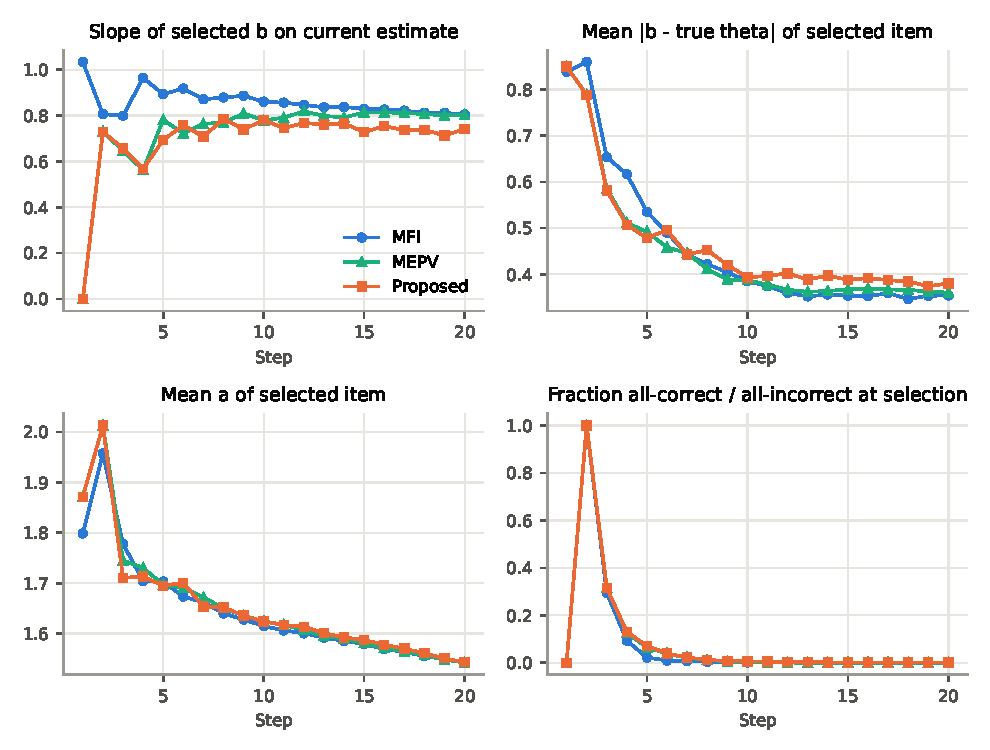
\includegraphics[width=\linewidth]{fig_selection.pdf}
\caption{選択された項目の特性のステップごとの推移}
\label{fig:selection}
\end{figure}

%% 報酬の尺度（reward_scale.csv，MFI の経路，2000人）: prec_gain 平均 s1 0.483，s5 0.582，s10 0.576，s20 0.540，s40 0.469；SD 0.061-0.187；負の割合 s40 0.0015（他 0）
%%   logvar 平均 s1 0.393，s5 0.170，s10 0.091，s20 0.045，s40 0.021；SD 0.041-0.053（s1-5），0.006（s40）
報酬の尺度については，MFIの経路に沿って計算した式\eqref{eq:reward}の報酬の平均はステップ1で0.48，ステップ5で0.58，ステップ40で0.47と，テストを通じて同程度であり，受験者間の標準偏差は0.06から0.19である．負の値をとる割合はステップ40で0.15\%，他のステップでは0であり，事後分散が増える反応は稀である．これに対し，事後分散の対数減少量の平均はステップ1の0.39からステップ40の0.02へ減少し，\ref{sec:reward}で述べた尺度の縮小が確認できる．

\subsection{推定モデルとデータ生成モデルが異なる場合の比較}\label{sec:misspecexp}

\ref{sec:misspec}の経路を確かめるため，データ生成モデルが推定モデルと異なる設定で比較した．データ生成モデルは，\ref{sec:expsetting}と同じ項目バンクの識別力と困難度に，擬似推測パラメータ$c_i\sim U(0.1,0.3)$を加えた3パラメータロジスティックモデル
\begin{equation}
 P_i(\theta)=c_i+\frac{1-c_i}{1+\exp\{-a_i(\theta-b_i)\}}
 \label{eq:3pl}
\end{equation}
とした．推定モデルは2PLMのままとし，全ての項目選択規則と式\eqref{eq:estimator}の推定量は真の識別力と困難度$(a_i,b_i)$を用いる．すなわち，項目パラメータに誤差はなく，推測という推定モデルに含まれない反応の成分だけが両モデルの差である．擬似推測パラメータは反復ごとに引き直し，評価用受験者の反応は式\eqref{eq:3pl}から生成した．提案手法は，学習時のシミュレーションにおける反応の生成と検証得点の算出にも式\eqref{eq:3pl}を用いた．これは，運用中の受験者と相互作用しながら学習する状況に対応する．各条件を反復4から6で実施した．

%% 転記元: ../Experiments/results/guess/table_rows.txt（make_tables.py guess；rep4-6.csv の平均と対応差）．2026-09-07 転記済み．
%% 対応差: 提案−MFI s3 −0.036 [−0.092,−0.003]，s5 −0.135 [−0.171,−0.116]，s10 −0.112，s20 −0.054，s40 −0.024 [−0.029,−0.015]（s3-40 いずれも 3/3負）；MEPV−MFI s5 −0.122，s40 −0.021 [−0.025,−0.015]（s3-40 3/3負）
%%   提案−MEPV s5 −0.013 [−0.022,+0.002] 混在，s10 −0.018 [−0.031,−0.002] 3/3負，s20 −0.005 [−0.010,+0.002] 混在，s30 −0.005 [−0.009,−0.001] 3/3負，s40 −0.003 [−0.004,−0.0001] 3/3負；提案−MPWI s40 −0.005 [−0.005,−0.005] 3/3負
実験結果を表\ref{tab:guess}に示す．表\ref{tab:guess}は，各ステップにおける真の能力に対するRMSEの3反復にわたる平均を項目選択規則ごとに示したものであり，最右列は使用した項目数の反復平均である．表では，ステップ3以降の各ステップの最良値を太字で示している．

\begin{table}[t]
\centering
\caption{推測を含むデータ生成モデルの下での各ステップにおけるRMSE（反復4から6の平均）}
\label{tab:guess}
\footnotesize
\setlength{\tabcolsep}{2pt}
\begin{tabular}{lcccccccc}
\hline
 & \multicolumn{7}{c}{ステップ} & \\
項目選択規則 & 1 & 3 & 5 & 10 & 20 & 30 & 40 & 項目数\\
\hline
MFI & 1.371 & 1.051 & 0.947 & 0.751 & 0.585 & 0.523 & 0.492 & 196\\
FIWL & 1.481 & 1.157 & 1.008 & 0.781 & 0.610 & 0.544 & 0.508 & 193\\
MPWI & 1.370 & \textbf{1.006} & 0.825 & 0.651 & 0.537 & 0.494 & 0.473 & 184\\
MEPV & 1.370 & \textbf{1.006} & 0.825 & 0.657 & 0.536 & 0.492 & 0.471 & 184\\
提案 & 1.370 & 1.015 & \textbf{0.812} & \textbf{0.639} & \textbf{0.531} & \textbf{0.487} & \textbf{0.468} & 156\\
\hline
\end{tabular}
\end{table}

表\ref{tab:guess}から，次のことがわかる．第一に，推測を含むデータ生成モデルの下では，推定モデルの下で最適な項目選択規則を含む全ての項目選択規則のRMSEが\ref{sec:expresult}より大きく，ステップ40でMFIは0.218から0.492へ，MEPVは0.220から0.471へ増加する．2PLMの推定量は推測による正答を能力の高さとして解釈するため，どの項目選択規則で項目を選んでも推定量の偏りは残る．その中で，事後分布に基づくMPWIとMEPVはステップ3以降の全てのステップでMFIを下回り，MEPVのMFIに対する対応差はステップ5で$-0.122$，ステップ40で$-0.021$（範囲$-0.025$から$-0.015$）と3反復の全てで負である．推定モデルがデータ生成モデルと一致する場合には終盤で消えていた事後分布に基づく項目選択規則の利点は，推測の下では終盤まで残る．

第二に，データ生成モデルから得た反応で学習した提案手法は，ステップ3以降の全てのステップでMFIを下回り（ステップ5で$-0.135$，ステップ40で$-0.024$，いずれも3反復の全てで負，ステップ40ではMFIの0.492の約5\%に相当），MEPVに対してもステップ10で$-0.018$（範囲$-0.031$から$-0.002$），ステップ30で$-0.005$，ステップ40で$-0.003$（範囲$-0.004$から$-0.0001$，MEPVの0.471の約1\%に相当）と3反復の全てで下回る．ステップ5と20では平均$-0.013$と$-0.005$であるが反復により符号が変わる．推定モデルがデータ生成モデルと一致する場合（表\ref{tab:main}）には提案手法とMEPVは同等であったのに対し，推測の下では提案手法がMEPVを小さいながら一貫して上回る．これは，\ref{sec:misspec}で述べた経路，すなわち提案手法が学習する期待精度増分が推測を含む実際の反応の分布の下で評価されることが，本設定で実際に働くことを示唆する．ただし，提案手法が改善するのは項目の選び方だけであり，推定量の偏りは残るため，改善の大きさは限定的である．以上の結果から，推定モデルとデータ生成モデルが異なる場合には，実際の反応から学習した提案手法が解析的な項目選択規則を上回ることが確認できた．

\subsection{推論時の選択時間}\label{sec:costexp}

各項目選択規則が1受験者の1ステップの項目選択に要する時間を計測した．10項目の反応履歴をもつ受験者に対し，受験者1人ずつ選択する場合と2000人を一括して選択する場合について，項目数$I$を500，2000，8000としたバンクで，1回の選択に要した壁時計時間を受験者数で割った値を求めた．提案手法は学習済みと同じ構造のネットワークを用い，状態の事後分散の計算を含めて計測した．計測はPyTorchとNumPyの線形代数ライブラリの双方でスレッド数を1に固定して行った．

%% 転記元: results/cost/cost.csv（make_tables.py cost の出力 results/cost/table_rows.txt）．2026-09-05 転記済み．
%%   Apple M系 CPU，torch 1 スレッド，OMP/OPENBLAS/MKL_NUM_THREADS=1，numpy 2.0.2；200回（1人）または5回（2000人）の平均．
計測結果を表\ref{tab:cost}に示す．表\ref{tab:cost}は，1受験者・1ステップあたりの選択時間をマイクロ秒で示したものである．

\begin{table}[t]
\centering
\caption{1受験者・1ステップあたりの選択時間（$\mu$s）}
\label{tab:cost}
\footnotesize
\begin{tabular}{lcccccc}
\hline
 & \multicolumn{3}{c}{受験者1人ずつ} & \multicolumn{3}{c}{2000人一括}\\
項目選択規則 & $I$=500 & 2000 & 8000 & 500 & 2000 & 8000\\
\hline
MFI & 7.1 & 14 & 45 & 2.5 & 10 & 44\\
FIWL & 36 & 40 & 59 & 8.8 & 11 & 19\\
MPWI & 36 & 40 & 59 & 8.8 & 11 & 19\\
MEPV & 53 & 79 & 390 & 11 & 20 & 57\\
提案 & 49 & 72 & 90 & 8.8 & 9.8 & 14\\
\hline
\end{tabular}
\end{table}

表\ref{tab:cost}から，次のことがわかる．第一に，いずれの項目選択規則も1受験者・1ステップの選択に要する時間は最大でも0.4msであり，本実験の規模では，事後分布に基づく項目選択規則を含めて実時間の運用に支障はない．格子上の事後分布の計算は行列積として一括で行えるため，1次元の能力に対しては計算量の問題は大きくない．第二に，項目数への依存は項目選択規則によって異なる．受験者1人ずつの選択では，項目数を500から8000へ増やすとMEPVは53$\mu$sから390$\mu$sへ約7倍になるのに対し，提案手法は49$\mu$sから90$\mu$sへ1.8倍にとどまり，MPWIは36$\mu$sから59$\mu$sである．項目数が小さい場合には，提案手法はネットワークの順伝播の固定的な費用のためMPWIより遅く，MEPVと同程度である．第三に，2000人を一括して選択する場合には，提案手法は項目数8000で14$\mu$sと最も速く，MEPVの57$\mu$sの4分の1程度である．以上から，提案手法の計算上の利点は，大規模なバンクにおける選択時間の伸びが1ステップ先の事後分散や事後精度を評価する項目選択規則より小さい点にあり，バンクが小さい場合の速度の利点は認められない．なお，多次元の能力を扱う場合には格子の点数が次元に対して指数的に増えるため事後分布に基づく項目選択規則の計算量が急増する．多次元の推定モデルの下での精度と選択時間は付録2で報告する．

\subsection{考察}\label{sec:discussion}

実験結果を踏まえ，提案手法の位置付けと適用範囲を整理する．第一に，推定モデルがデータ生成モデルと一致する場合，提案手法は事後分布に基づく解析的な項目選択規則と同等の精度にとどまり，それを上回らなかった（\ref{sec:expresult}）．提案手法の目的はMEPVの目的と同一ではなく（\ref{sec:reward}），両者の選択が常に一致するわけではないが，本実験の設定では精度は同程度であった．推定モデルが正しければ，提案手法が学習する式\eqref{eq:reward}の報酬の条件付き期待値は推定モデルの下で計算できる量であり（\ref{sec:misspec}），この場合に学習によって得られるのはその量の近似である．したがって，項目数の大きいバンクにおける選択時間の利点（\ref{sec:costexp}）を除けば，この場合に学習を用いる積極的な理由はない．第二に，データ生成モデルが推測を含む場合には，実際の反応から学習した提案手法が解析的な項目選択規則を小さいながら一貫して上回った（\ref{sec:misspecexp}）．この優位は，報酬の期待値が実際の反応の分布の下で評価されることによるものであり，推定モデルの誤りによる推定量の偏りそのものは解消しない．したがって，提案手法の利点は，推定モデルがデータ生成モデルと異なる状況で項目の選び方を改善する点にあり，その大きさは両モデルの差の種類と程度に依存する．第三に，提案手法が学習するのは，学習集団の能力分布と探索方策の下での報酬の期待値であり，得られる方策は学習集団に依存する．また，状態は反応履歴の要約であって履歴そのものではなく，尤度の非対称性などは失われる．反応履歴を状態に含めても精度が改善しないことは付録1で確かめたが，本論文の実験は，2PLM，単一の項目バンク，固定長のテスト，及び式\eqref{eq:estimator}の推定量という条件の下での比較であり，結果をこの条件の外へそのまま一般化することはできない点に留意されたい．

\section{むすび}\label{sec:conclusion}

本論文では，深層Q学習に基づくCATの項目選択法について，全パラメータの非負制約，能力推定値だけを用いる状態，及び選択時の推定値における情報量という報酬に関する既存手法の問題点を整理し，最尤推定値，テストの進行度，事後分散からなる状態と，事後精度の増分という推定値の不確実性を考慮した報酬に基づく項目選択法を提案した．また，2PLMに基づくシミュレーション実験により，提案手法がテスト序盤でMFIを上回り，事後分布に基づく解析的な項目選択規則と同等の精度を，候補項目ごとの期待値計算を学習したQ関数で置き換えて達成すること，既存手法の劣化の決定的な要因が非負制約であり学習設定がそれに次ぐこと，反応履歴から計算できる報酬の中では事後精度の増分が有効で割引率は0から0.5で同等であること，及び事後分散を状態に含めることの寄与はテスト序盤に限られ小さいことを示した．更に，データ生成モデルが推測を含む一方で推定モデルが2PLMである場合には，実際の反応から学習した提案手法が解析的な項目選択規則を小さいながら一貫して上回ることを示した．付録では，反応履歴を状態に含める定式化が精度を改善しないこと，2次元のデータ生成モデルの下で学習した方策が解析的な項目選択規則を上回るのは項目パラメータの推定誤差が出題次元の偏りを生む場合に限られること，及び推定モデルとデータ生成モデルが一致する多次元の項目反応モデルの下では学習した方策が厳密な近視眼的な項目選択規則を上回らないことを，再現に必要な設定とともに報告した．

なお，本研究では推定モデルを2PLMに限り，単一のバンクと固定長のテストのみを扱ったが，複数のバンク，可変長の終了規則，露出制御や内容制約を伴う設定への拡張は今後の課題としたい．また，推定モデルとデータ生成モデルの差は推測に限り，学習はデータ生成モデルとの相互作用を仮定したが，他の差の下での挙動や，固定された過去の記録だけから学習する場合への拡張も今後の課題としたい．

\bibliographystyle{sieicej}
\bibliography{references}

\appendix
\section{反応履歴を状態に含める定式化の検討}\label{app:history}

本文の提案手法は，推定モデルの下で計算される状態と報酬を用いる．これに対し，反応履歴そのものを状態に含める履歴状態と，パラメータ推定に用いた反応データから学習する方式を，推定モデルとデータ生成モデルの差が本文より大きい設定で検討した．本付録では，再現に必要な設定と主要な結果を要約する．数値は反復6から10の平均である．

%% 転記元: appendix_sources/HistoryDQN/（main.tex の 6.1〜6.9 節，mirt_rows_guess.txt，table_rows_ref.txt，combined_rows.txt，rows.txt，summary_conf.txt）．2026-09-08 転記（参照報酬・MEMSE・予測器の記述は削除）．
設定は次のとおりである．データ生成モデルは，本文と同じ識別力と困難度をもつ500項目を二つの次元へ250項目ずつ無作為に割り当て，項目$i$の属する次元を$d(i)\in\{1,2\}$，受験者の能力を$(\theta_{j1},\theta_{j2})$として，正答確率を$c_i+(1-c_i)/[1+\exp\{-a_i(\theta_{j,d(i)}-b_i)\}]$，$c_i\sim U(0.1,0.3)$とする2次元単純構造の項目反応モデル~\cite{Reckase2009}とし，能力は平均0，分散1，相関$\rho\in\{1,0.9,0.7,0.5,0.3\}$の2変量正規分布から生成した．推定モデルは2PLMとし，その項目パラメータは，パラメータ推定用の受験者5000人が全項目に回答した反応データから，母集団分布を$N(0,1)$とする周辺最尤法~\cite{BockAitkin1981}により格子上のEMアルゴリズムで推定した．真の能力が2次元であるため，評価の基準には，各受験者のバンクの全項目への反応から推定したパラメータと式\eqref{eq:estimator}で求めた能力推定値（以下，全項目推定値）を用い，これに対するRMSEを報告した．評価用受験者は反復ごとに2000人，テスト長は40，反復$k$の乱数種は$20260904+k-1$とし，反復1から5を設計の選択に，6から10を評価に用いた．DQNの学習設定は本文の提案手法と同じである．推定モデルがデータ生成モデルと一致する一次元の設定（本文と同じバンクと2PLM）も同じ乱数種で併せて実施した．

比較した条件は，状態が式\eqref{eq:state}の状態と履歴状態（式\eqref{eq:state}の状態に出題済み指示ベクトルと正答指示ベクトルを連結した$3+2I$次元）の二通り，学習方式が通常のDQN（$\gamma=0.5$）と全候補項目への回帰の二通りであり，報酬はいずれも式\eqref{eq:reward}である．全候補項目への回帰は，パラメータ推定用の反応データの各受験者が全項目への反応をもつことを利用し，各ステップで全ての候補項目$i\in\mathcal{B}_{jt}$について反実仮想の反応と報酬$r_{jt}(i)$を計算し，$\gamma=0$の下で損失$|\mathcal{B}_{jt}|^{-1}\sum_{i\in\mathcal{B}_{jt}}\{Q(s_{jt},i;\bm{w})-r_{jt}(i)\}^2$を再生メモリ上で最小化する学習であり，目標ネットワークとブートストラップを用いない．反実仮想の推定値は，履歴の対数尤度に候補項目の対数尤度を加えた関数を$[-4,4]$上の161点の格子で評価し，最大点の近傍の二次補間で求めた．設計の選択の段階では，このほかに直近8項目の8次元埋め込みと反応符号を連結した状態，及びゲート付き再帰ユニット（32次元）で履歴を要約した状態を検討したが，いずれも出題済みと正答の指示ベクトルによる履歴状態を上回らなかった．

%% 表の数値: appendix_sources/HistoryDQN/main.tex の表（反復6-10，rmse_ref s40）と table_rows_ref.txt（uni）．列順 MFI, belief, belief_all, history_prec．
主要な結果を表\ref{tab:app-mirt}に示す．表\ref{tab:app-mirt}は，一次元の設定と2次元の設定の各相関について，ステップ40における全項目推定値に対するRMSEの反復6から10にわたる平均を示したものであり，「通常」は式\eqref{eq:state}の状態を通常のDQNで学習した条件，「回帰」は同じ状態を全候補項目への回帰で学習した条件，「履歴」は履歴状態を全候補項目への回帰で学習した条件を表す．

\begin{table}[t]
\centering
\caption{一次元及び2次元のデータ生成モデルの下でのステップ40の全項目推定値に対するRMSE（反復6から10の平均）}
\label{tab:app-mirt}
\footnotesize
\setlength{\tabcolsep}{4pt}
\begin{tabular}{lcccc}
\hline
設定 & MFI & 通常 & 回帰 & 履歴\\
\hline
一次元 & 0.199 & 0.200 & 0.198 & 0.197\\
$\rho=1$ & 0.265 & 0.268 & 0.262 & 0.259\\
$\rho=0.9$ & 0.269 & 0.279 & 0.267 & 0.269\\
$\rho=0.7$ & 0.285 & 0.281 & 0.280 & 0.306\\
$\rho=0.5$ & 0.324 & 0.321 & 0.310 & 0.356\\
$\rho=0.3$ & 0.408 & 0.374 & 0.364 & 0.419\\
\hline
\end{tabular}
\end{table}

%% 対応差（s40，反復6-10，MFI 基準で記録があるもの）: 一次元 回帰−MFI −0.0006 [−0.002,+0.001] 混在，通常−MFI +0.001 混在，履歴−MFI −0.002 [−0.003,−0.0005] 5/5負．2次元の回帰−MFI の反復別の符号は記録がなく，平均値の差だけを述べる．
%%   探索（反復1-5，s40，ρ=0.5）: MFI 0.295，回帰 0.298（combined_rows.txt）
%%   均衡上界（MFI，balanced−plain s40）: 反復6-10 ρ=0.5 −0.033 [−0.062,−0.011] 5/5負，ρ=0.3 −0.102（反復別 −0.084/−0.178/−0.190/−0.027/−0.029）5/5負（summary_conf.txt）
%%   反復8 ρ=0.3 第1次元割合 MFI 0.829 / 回帰 0.786（NOTES_design_options.md）；有限標本 ρ=0.3 s40 回帰 500人 0.380，1000人 0.374，4500人 0.366（MFI 0.408）；頑健性 rows.txt（MFI と回帰の平均値）
表\ref{tab:app-mirt}から，次のことがわかる．第一に，推定モデルがデータ生成モデルと一致する一次元の設定では，履歴状態は精度を改善せず，全ての条件がMFIと0.002以内で一致する．これは，データ生成モデルが推定モデルに一致するとき，報酬の条件付き期待値が事後分布の関数となり，履歴状態が式\eqref{eq:state}の状態に加える情報は事後分布の要約の精緻化にとどまるためである．第二に，2次元の設定では，式\eqref{eq:state}の状態を全候補項目への回帰で学習した条件のRMSEが，$\rho=0.7$で0.280，$\rho=0.5$で0.310，$\rho=0.3$で0.364と，MFIの0.285，0.324，0.408より小さく，相関が小さいほど差が広がる．一方，履歴状態は同じ学習方式でも式\eqref{eq:state}の状態より$\rho=0.7$で0.026，$\rho=0.5$で0.046，$\rho=0.3$で0.055大きく，MFIにも及ばない．表現力の高い状態は，推定モデルの下で計算される報酬という誤った目的をより強く最適化する分だけ，全項目推定値の再現を損なうと考えられる．

第三に，2次元の設定における全候補項目への回帰の優位は，項目パラメータの推定誤差が出題次元の偏りを生む場合に限って現れる．パラメータ推定用の反応データによっては一方の次元の項目の識別力が過大に推定され，MFIは出題の83\%をその次元に偏らせる（$\rho=0.3$の反復8）のに対し，回帰は79\%であった．真の次元ラベルを用いて出題数の少ない次元の項目だけを候補とする均衡制約をMFIに課すと，ステップ40のRMSEは反復6から10の平均で$\rho=0.5$で0.033，$\rho=0.3$で0.102小さくなり（いずれも5反復の全てで負），$\rho=0.3$の改善は反復により0.027から0.190まで変動した．すなわち，推定誤差が生む偏りとそれによる誤差の大きさはパラメータ推定用の反応データに強く依存し，回帰の優位はこの偏りが大きい反復に集中した．設計の選択に用いた反復1から5の$\rho=0.5$では偏りが小さく，回帰はMFIを上回っていない（0.298対0.295）．パラメータ推定用の反応データだけから学習した場合も$\rho=0.3$のステップ40で500人のデータで0.380，1000人で0.374，4500人で0.366（MFIは0.408）であり，バンクの生成分布，項目数，テスト長を変えた変種でも，一次元では回帰とMFIの差は0.002以内，$\rho=0.3$では回帰がMFIより0.010から0.041小さかった．

以上から，反応履歴を状態に含めても精度は改善せず，本文の式\eqref{eq:state}の状態と式\eqref{eq:reward}の報酬の組合せが，実際の反応から学習する限りにおいて最も有効であることが確認できる．本文\ref{sec:misspecexp}の推測の下での提案手法の優位と，2次元のデータ生成モデルの下での全候補項目への回帰の優位は，いずれも推定モデルの下で計算される報酬の期待値を実際の反応の分布の下で学習することによる．その大きさは，解析的な項目選択規則が推定モデルの下で計算する期待値と実際の期待値の食い違いの大きさに依存し，保証されるものではない．

\section{多次元の推定モデルの下での検討}\label{app:mirt}

データ生成モデルと推定モデルがともに補償型の多次元ロジスティックモデル$P_{ij}=1/[1+\exp\{-(\bm{a}_i^{\top}\bm{\theta}_j+d_i)\}]$である推定モデルとデータ生成モデルが一致する多次元のCATにおいて，深層Q学習が厳密に計算した近視眼的な解析的項目選択規則を上回るかを検討した．Liらは，事後分散に基づく報酬の深層Q学習が近視眼的な項目選択規則より少ない項目数で所定の事後分散に到達することを報告している~\cite{LiGibbonsRockova2026}．しかし，比較対象の項目選択規則は事後分布をモンテカルロ近似で評価していたため，改善が近視眼性の克服によるのか近似の粗さによるのかは明らかでなかった．

%% 転記元: appendix_sources/MIRTDQN/（main.tex，main_k2_cross_table_rows.txt，main_k2_target1_table_rows.txt，main_k3_bifactor_table_rows.txt，explore_k2_cross_table_rows.txt，table_rows.txt（選択時間））．2026-09-07 転記済み．
設定は次のとおりである．第一のシナリオは$K=2$，事前分布の相関0.5，500項目とし，各項目の主次元を無作為に割り当て，主識別力を$U(0.6,2.0)$，半数の項目に副次元の識別力$U(0.2,1.0)$を与え，切片$d_i$を$U(-2,2)$から生成した．対象次元を両次元とする設定と，次元1だけを対象とし次元2を妨害次元とする設定を設けた．第二のシナリオは$K=3$，直交な事前分布とし，全ての項目が一般因子に$U(0.6,2.0)$の識別力をもち，二つの特殊因子のいずれか一方に$U(0.4,1.4)$の識別力をもつ双因子構造で，対象は一般因子のみである．事後分布は$[-3.5,3.5]^K$上の各次元51点（$K=2$）又は33点（$K=3$）の格子で厳密に計算し，推定量は事後平均とした．評価指標は，対象次元のRMSE（最大長40の固定長）と，対象次元の事後分散が閾値0.16（事後標準偏差0.4，Liらと同じ）を下回るまでの平均項目数である．評価用受験者は反復ごとに2000人，反復$k$の乱数種は$20260906+k-1$とし，反復1から5を設計の選択に，6から10を評価に用いた．比較した近視眼的な項目選択規則は，D最適~\cite{Segall1996}，A最適とその対象次元限定版である$D_s$最適~\cite{MulderVanderLinden2009}，最小期待事後分散（MEPV）~\cite{vanderLinden1999}とその最大分散版（MEMV），KL情報量~\cite{VeldkampVanderLinden2002}，相互情報量~\cite{WangChang2011}，並びに妨害次元がある場合のKL情報量と相互情報量の対象次元限定版である．深層Q学習の状態は，事後平均，事後分散の対数，事後相関，及び進行度からなる状態とし，報酬は対象次元の事後精度の和の増分，事後分散の和の減少量，最大分散の減少量，及び閾値に達するまで各ステップに$-1$を与える終了報酬~\cite{LiGibbonsRockova2026}の4種類，学習方式は付録1の全候補項目への回帰（$\gamma=0$）と通常のDQN（$\gamma=0.9$，終了報酬では$0.95$）とし，Double DQN~\cite{vanHasselt2016}と本文と同じ学習設定を用いた．学習に基づく方策が近視眼的な項目選択規則を上回ると判断する基準は，実験に先立ち，最良の学習方策と最良の近視眼的な項目選択規則の対応差がステップ20と40の双方で5反復の全てで負かつ平均$-0.005$以下であること，及び終了までの項目数の差が5反復の全てで負かつ$-0.5$項目以下であることと定めた．

%% 表の数値: main_k2_cross_table_rows.txt，main_k2_target1_table_rows.txt，main_k3_bifactor_table_rows.txt（反復6-10）．
主要な結果を表\ref{tab:app-k}に示す．表\ref{tab:app-k}は，各設定について，ステップ40における対象次元のRMSEと終了までの平均項目数の反復6から10にわたる平均を示したものである．

\begin{table}[t]
\centering
\caption{推定モデルとデータ生成モデルが一致する多次元の項目反応モデルの下でのステップ40のRMSEと終了項目数（反復6から10の平均）}
\label{tab:app-k}
\scriptsize
\setlength{\tabcolsep}{1.5pt}
\begin{tabular}{@{}lcccccc@{}}
\hline
 & \multicolumn{2}{c}{$K=2$，両次元} & \multicolumn{2}{c}{$K=2$，妨害} & \multicolumn{2}{c}{$K=3$，双因子}\\
項目選択規則・条件 & RMSE & 項目 & RMSE & 項目 & RMSE & 項目\\
\hline
D最適（非限定） & 0.264 & 17.5 & 0.260 & 15.0 & 0.368 & 29.6\\
A最適（対象） & 0.264 & 16.7 & 0.207 & 8.3 & 0.294 & 12.2\\
MEPV（対象） & 0.265 & 16.6 & 0.207 & 8.3 & 0.295 & 12.2\\
精度増分・回帰 & 0.283 & 27.1 & 0.207 & 8.4 & 0.297 & 12.3\\
分散減少・回帰 & 0.279 & 17.5 & 0.228 & 8.5 & 0.310 & 12.6\\
精度増分・$\gamma=0.9$ & 0.286 & 24.4 & 0.212 & 9.2 & 0.301 & 13.3\\
分散減少・$\gamma=0.9$ & 0.324 & 23.9 & 0.280 & 13.1 & 0.356 & 20.5\\
終了報酬・$\gamma=0.95$ & 0.305 & 19.8 & 0.245 & 9.5 & 0.328 & 14.6\\
\hline
\end{tabular}
\end{table}

%% 対応差: K=2 両次元 分散減少回帰−A最適 s40 +0.015 [+0.010,+0.022] 5/5正，終了 +0.80 [+0.52,+1.33] 5/5正；終了報酬 終了 +3.19 [+2.41,+3.54] 5/5正
%%   K=2 妨害 精度増分回帰−MEPV s40 −0.0002 [−0.005,+0.003] 混在，終了 +0.09 [+0.01,+0.18] 5/5正；γ=0.9 +0.006 [+0.001,+0.010] 5/5正，終了 +0.91；終了報酬 終了 +1.15 [+1.00,+1.38] 5/5正
%%   K=3 精度増分回帰−MEPV s40 +0.002 [−0.0000,+0.005] 混在，終了 +0.07 [+0.03,+0.15] 5/5正；分散減少回帰 +0.016 5/5正；γ=0.9 +0.006 5/5正，終了 +1.14；終了報酬 +0.033，終了 +2.43 [+2.15,+2.66] 5/5正
%%   選択時間（1人ずつ，K=3，I=2000）: MEPV 76577 \UTF{00B5}s，KL 25275，MI 37854，D最適 97，A最適 59，DQN 49；K=2，I=500: MEPV 1092，DQN 32
表\ref{tab:app-k}と対応差から，次のことがわかる．第一に，対象次元が複数の場合には，A最適，D最適，MEPV，KL情報量，相互情報量がステップ40で0.264から0.265，終了までの項目数で16.6から17.5項目と同等に最良である．最良の学習方策である分散減少・回帰は，A最適に対してステップ40で$+0.015$（範囲$+0.010$から$+0.022$），終了までの項目数で$+0.80$項目（範囲$+0.52$から$+1.33$）と，いずれも5反復の全てで劣る．第二に，妨害次元がある場合には，対象次元に限定した近視眼的な項目選択規則（$D_s$最適，A最適，MEPV，MEMV，相互情報量の対象限定版）が0.207，8.3項目で一致して最良であり，対象を限定しないD最適，KL情報量，相互情報量は0.260，15.0項目と大きく劣る．精度増分・回帰はMEPVとの対応差がステップ40で$-0.0002$と符号が混在し，終了までの項目数は$+0.09$項目（5反復の全てで正）である．3次元の双因子構造でも同様であり，精度増分・回帰はMEPVに対して$+0.002$（範囲$-0.0000$から$+0.005$，符号は混在），終了で$+0.07$項目（5反復の全てで正）である．すなわち，学習した近視眼的方策は対象次元に限定した厳密な近視眼的な項目選択規則と同等の精度に達するが，それを上回らない．第三に，割引率を正とする非近視眼的な学習はどの報酬でも近視眼的な学習より劣り（精度増分で$\rho$によらず$+0.006$，5反復の全てで正），終了報酬の学習は終了までの項目数が近視眼的な項目選択規則より1.15項目（妨害次元あり）から3.19項目（両次元）多い（いずれも5反復の全てで正）．実験に先立ち定めた基準はいずれの設定でも満たされなかった．

以上から，推定モデルとデータ生成モデルが一致する多次元の項目反応モデルの下では，学習に基づく項目選択が厳密な近視眼的な項目選択規則を上回る証拠は得られず，Liらが報告した項目数の削減は，比較対象の項目選択規則が事後分布を近似的に評価していたことによる可能性がある．選択時間については，いずれの項目選択規則も反応後の事後分布の更新を除いた選択の計算だけを計測したところ，1ステップ先の事後分布のモーメントを候補項目ごとに求めるMEPVが格子点数と項目数の積に比例して増え，$K=3$，2000項目で受験者1人あたり76msに達するのに対し，本文と同じ状態のDQNは次元数と格子点数によらず49$\mu$sであった．したがって，多次元の推定モデルの下での学習に基づく項目選択の利点は精度ではなく，格子上の事後分布に基づく項目選択規則の計算が困難になる高次元での計算量にある．本文と本付録の結果を併せると，学習に基づく項目選択が解析的な項目選択規則を精度で上回るのは，推定モデルが正しい場合ではなく，推定モデルとデータ生成モデルが食い違い，解析的な項目選択規則が誤った推定モデルの下で期待値を計算せざるを得ない場合に限られる．


\end{document}
